\subsection{Introduktion}
Kasseapparatet er et program som viser produkter og kan håndtere disse i en indkøbskurv, samt herfra gennemføre salg og danne salgskvitteringer. Produkterne som vises i kasseapparatet hentes fra Centralserveren\footnote{Se beskrivelse af systempakker på figur \ref{fig:system_oversigt}, side \pageref{fig:system_oversigt}}. De viste produkter i kasseapparatet opdateres ikke for hver ændring i produkter i CentralServer, men når en ekspedient beder om en opdatering manuelt. Denne funktionalitet er valgt, da det ikke var ønsket at produkter kom frem og forsvandt under brug af systemet. Da dette ville være forstyrrende for en ekspedient.


\subsection{Design og struktur}
Kasseapparatet er designet med MVVM~\cite{MVVM}, med stor fokus på adskilelse af Forretningslag og Præsentationslaget. Dette er sikret ved brug af klasser der står for at styre logikken i grænsefladen samt kommunikere ned i de nedre lag, disse kaldet viewmodels. Disse bliver forklaret nærmere længere nede i kapitel ?.
Vores system er herunder beskrevet ved følgende pakkediagram.	

\begin{figure}[H]
	\centering
	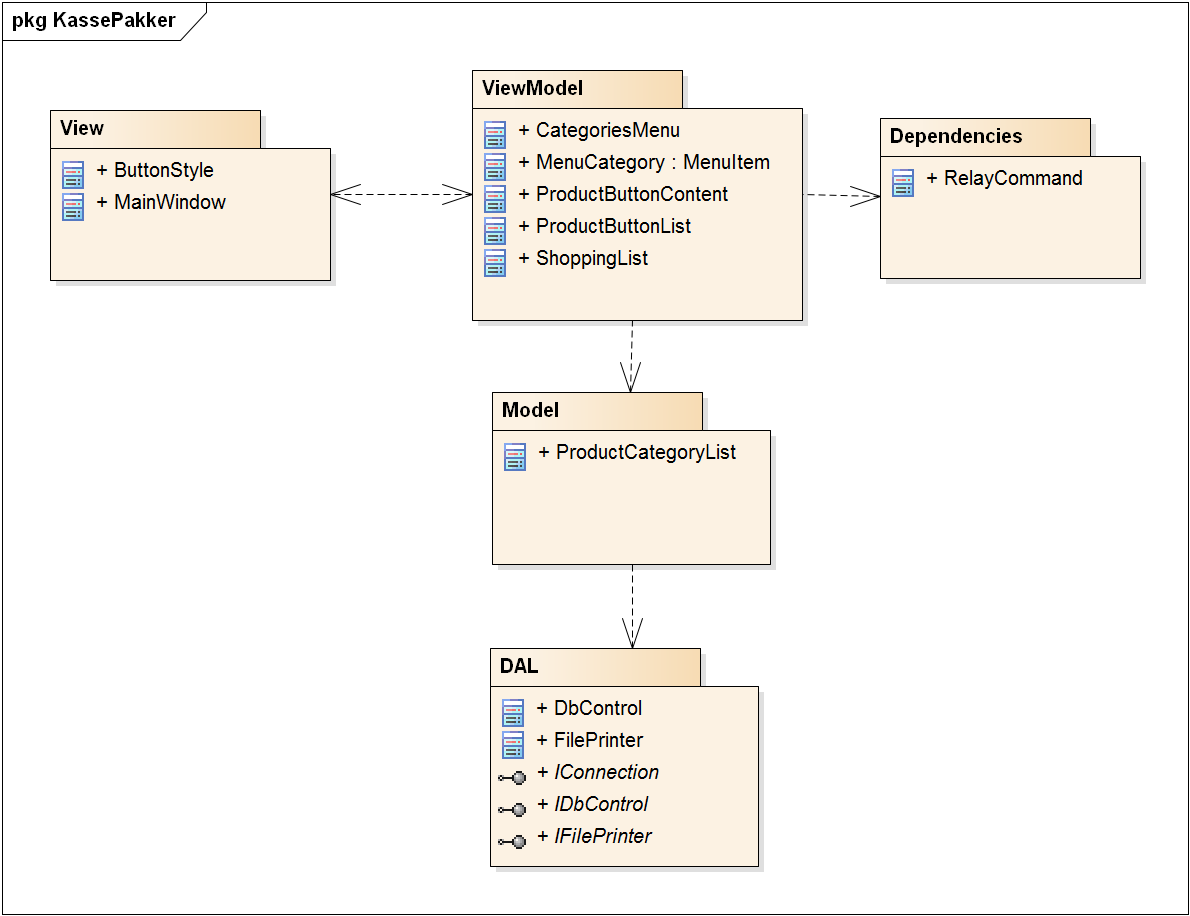
\includegraphics[width=0.8\textwidth]{Systemdesign/Frontend/pics/KassePakker}eG
	\caption{Pakkediagram over kasseapparat.}
	\label{fig:EndeligUI}
\end{figure}

Som man kan se på det ovenstående pakkediagram består kasseapparatet primært af grænsefladen og et data access lag. Dette er fordi at kasse apparatet ikke har som ansvar at kunne oprette/ redigere og slette produkter, men bare at afspejle produkterne i databasen. 

\begin{itemize}
	\item \textbf{View} Views indeholder vores præsentationslagslogik. Det er skrevet i XML og er direkte med til at style vores grænseflade.
	\item \textbf{ViewModel} Er en mediator mellem modellaget og grænsefladen. Viewmodels sikrer at kasseapparatets grænseflade afspejler ændringer der sker nede i systemet, samt kommunikerer grænsefladens ændringer til de lavere lag.
	\item \textbf{Dependencies} Indeholder sourcekode der gør det nemmere at arbejde med commands.
	\item \textbf{Model} Indeholder business logic. Dette er der ikke særligt meget af, da det meste business logic er styret fra administrationssystemet.
	\item \textbf{DAL} Indeholder logik til at kommunikere med CentralServeren og derved Databasen.
\end{itemize}
